
\documentclass[journal]{IEEEtran}
\hyphenation{op-tical net-works semi-conduc-tor}
\usepackage{amsfonts}
\usepackage{amsmath}
\usepackage{enumerate}
\usepackage{algorithm}
\usepackage{caption}
\usepackage{algpseudocode}
\usepackage{listings} 
\usepackage{graphicx}
\usepackage{pseudocode}
\usepackage[noae]{Sweave}
\usepackage{hyperref}
\begin{document}

\title{What and When of Random Forest}

\author{Debpriya~Seal\\,% <-this % stops a space
\IEEEauthorblockA{School~of~Informatics~and~Computing\\
Indiana~University\\
Bloomington,~Indiana~47405-7000\\
Email: debseal@indiana.edu}
\thanks{Prof. M Dailklic with Indiana University for consistent support and encouragement}% <-this % stops a space
}

% The paper headers
\markboth{B565: Data Mining, Assignment V}%
{B565: Data Mining, Assignment V}
\maketitle


\begin{abstract}
%\boldmath
Random Forest has been in highlight lately. Argueably it is best classifiction algorithm we have. This paper provides a light introduction to Random forest. This paper starts with the basics, and then will show to application of the same in R with a toy example. 
\end{abstract}
\begin{IEEEkeywords}
Random Forest, Bootstrap Aggregation/Bagging, R
\end{IEEEkeywords}

\IEEEpeerreviewmaketitle

\section{Introduction}

\subsection{For a layman}
\IEEEPARstart{R}{andom} Forest  is a learning method to classify or predict the values of objects. However, it is a bit different from the usual methods which predicts or classify objects. In general, there is this one classifier which classifies/predicts objects. However, in random forest we make bunch of them, and try to keep them as different as possible by imputing randomness. And the classifier we use are decision trees. Hence, random + forest i.e random forest.
\subsection{Formally}
\IEEEPARstart{R}{andom} forest is ensemble learning method used for classification (or regression). There are 2 terms we need to know before we go any further with Random forest is Decision trees and ensemble Methods. Let first understand them briefly.

\subsubsection{Decision trees}
Decision Trees is a classifcation algorithm. Later on, you will see that Random forest is nothing but a bunch of decision trees put together.Decision tree, the name has it. It is an algorithm in which we create a tree to classify objects. An input enters enter the top of the tree and as it traverse down the tree, the input data gets bucketed into smaller and smaller sets, to reach a leaf node which predicts the class/category it belongs to.

\subsubsection{Ensemble Methods}
This is method to improve the classification accuracy. It uses the divide-and-conquer approach.  The basic idea is that a group of ``	weak learners" come together to form a ``strong learner". And the way this is achieved is by building bunch of classifier, and then using the prediction from each of them together to come up with the final prediction. The idea is simple, that one classifier may go wrong, 2 may go wrong, but not all of them can go wrong. And we classfiy a test object to be the one which is the majority of all. Now you can create ensemble of classfiers in many way:
\begin{enumerate}
	\item \textbf{Using Training datasets}: In this method we resample from the given training set based on some sampling distribution. Boosting and Bagging are the example of ensemble methods which uses training datasets.
	\item \textbf{Using Input Features}: In this we rather using  different trainings records, we use different subset of features to train different classifiers.
	\item \textbf{Using Class Labels}: This method is used when you tons of class labels. You divide the labels into 2 binary class. And then train on these two labels. You perform this recursively.
	\item \textbf{Using learning algortihm}: There are learning algorithms in which you can tweak the algortihm to has classifiers react different. Typical example would be that of NN (Neural Network). By changing the weights attached to each link, you can get a classfier behave different. Similarly, with decision trees, instead of choosing the best feature, choose randomly between the top $i^th$ randomly
\end{enumerate}

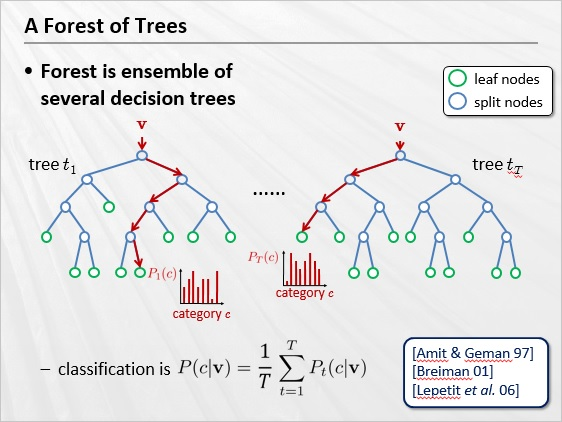
\includegraphics[width=3.25in,height=3.25in,clip,keepaspectratio]{RandomForest.jpg}
% needed in second column of first page if using \IEEEpubid
%\IEEEpubidadjcol

Now, Random forest is an amalgamation of the above 2 ideas (i.e. Decision Trees and Ensemble methods). We make bunch of Decision trees(our weak learner).And then we get the prediction from each of the decision trees. And now maybe the forest starts to make more sense. And the Random forest is the strong leaner, which predicts the class which majority of the decision trees predicted.However, it should not be difficult ot see that you want these individual trees (decision trees) to as different as possible. Since, if they are identical, then there is no difference between your tree and random forest. The term random refers to the randomness you would like to keep in these individual decision trees. \\
Now, you would be thinking what is this randomness we are talking about in the random forest. So, there are 2 type of randomness we incorporate in Random Forest:
\begin{enumerate}[a.]
	\item \textbf{Boostrap Aggregation(or Bagging)}: \emph{Boostrap Aggregation(or Bagging)} is a ensemble technique in which we repeatedly  re-sample (say N times) with replacement, according to some unfiorm probability distribution. We this to pick different set of training dataset for each classifer $C_{k}$.
	\item \textbf{Random subspace}: Once we get the training dataset $D_{k}$. At each node, we know randomly pick say f subset features from the set of feature F. And then based on some measure (entropy, genie etc.) we pick the best feautre from these f subset of feature and not complete F set of features. Small number of f, may decrease you chances of trees being correlated .On the other hand, big number of features gives your tree more strenght. So as a thumb rule $f = \log_2F+1$ where F is the total number of features.
\end{enumerate}
Also to measure the error of random forest, below equation is used:
\begin{eqnarray}
Generalization Error &\le&  \frac{\bar{\rho}(1-s^2)}{s^2}
\end{eqnarray}
where $\bar{\rho}$ is the average correlation between the different trees and $s$ is the strength of the tree.The above equation is pretty much straightforward. You would not want to have an correlation between any of your individual trees. If you have more identical trees then the bound of the generalization error tends to increase.
Below is a pseudo-code for the Random Forest:
\begin{algorithm}
\renewcommand\thealgorithm{}
\caption{Random Forest}\label{RandomForest}
\begin{algorithmic}[1]
	\State Let D be \{($x_1,y_1$),($x_2,y_2$),($x_3,y_3$), \ldots ,($x_n,y_n$)\}	
	\State Let $x_i \in \mathbb{R}^F$  i.e. $x_i = \{a_1, a_2,a_3, \ldots,a_F\}$
	\State Let $c$ be the number so classifiers we intend to make
	\For{$i = 1 \ldots c$} 
		\State Choose a bootstrap sample $D_i$ from D
		\State Train a classifier on $D_i$ dataset such that:
		\State \hspace{\algorithmicindent} a) You do not prune the tree, and let grow fully.
		\State \hspace{\algorithmicindent} b) For each node, randomly pick f subset features of 
		\State \hspace{\algorithmicindent} features i.e. $f < F$
	\EndFor
	\For{each test data i } 
		\State Test it on all $c$ classifier and pick majority 
		\State votes for classifcation (or average for regression)
	\EndFor
 \end{algorithmic}
\end{algorithm}	

\section{Toy Example To Illustrate}
Lets try to understand the concept with a toy example.
		\begin{table}[h]
			\caption{Dataset for Classification} 
			\centering
			\begin{tabular}{cccc| r}
				\hline \\
				S.No. & Fever & Nausea & Weakness & Viral \\
				\hline 
				1 & 0 & 0 & Mild & N \\
				2 & 0 & 1 & High & N \\
				3 & 1 & 0 & Low & Y \\
				4 & 1 & 1 & Mild & Y \\
				5 & 1 & 0 & High & N \\
				6 & 1 & 1 & High & Y \\
				\hline
			\end{tabular}	
		\end{table}	
Lets take an example in which we are trying to predict wether a person has fever or not based on 3 sypmtoms. Lets see how random forest will work on this.
\begin{enumerate}[Step 1:]
	\item Sample N records (say 2) from the above dataset (with replacement).
	\item Assuming we are making forest of 2 decision trees. For the first tree we sampled records 1 and 2. Clearly we can see that it will have root and leaf node straight away. As for both of it cases, we have the class to be N.\\
	Similarly, suppose we pick records 3,4 and 5 for the second tree and here as well everything is Y. So again we get the same tree.
	\item Given a test record we ask all the above tree and we take the majority. So this is how classification works in Random Forest.
\end{enumerate}
\section{Application in R}
R already has a inbuild package to implement Random forest. And as the first step you would like to install the same. Below is how you can do so:
\begin{Schunk}
\begin{Sinput}
> install.packages("randomForest")
\end{Sinput}
\end{Schunk}
Once you have the library installed, you should load the package.And below is how you do that.
\begin{Schunk} 
\begin{Sinput}
> library("randomForest")
\end{Sinput} 
\end{Schunk}
\textbf{NOTE:} You could also require("randomForest"). The only difference being, library() throws an error if the library is not found. However, require() does not, hence require is generally used in functions more often. \\
The next thing is to get some kind of dataset to train/test random Forest. We will use the $iris$ dataset, which comes in default with almost all R installations. So the only thing you need to do is load the dataset. Below is how you can do so:
\begin{Schunk} 
\begin{Sinput} 
> load(iris)  
\end{Sinput} 
\end{Schunk}
Now lets create training adn test dataset out of it.
\begin{Schunk} 
\begin{Sinput} 
> train = sample (1:nrow(iris),nrow(iris)/2)
> test = iris[ c(1:100), ]
\end{Sinput} 
\end{Schunk}
And now we call the real function i.e. $randomForest$. Below is how we call it.
\begin{Schunk} 
\begin{Sinput} 
> iris.train = randomForest(Species ~., data=train, 
importance=TRUE, do.trace=100)
\end{Sinput} 
\end{Schunk}
Lets discuss the arguments of randomForest:
\begin{enumerate}
	\item $data:$ Here you mention the dataset you want to be used for training.
	\item $importance:$ It takes a boolean value, were you mention that you would like to assess the importance of feature.
	\item $do.trace:$ It is to set the verbose mode on/off.
	\item $mtry:$ In random forest the number of features selected is a factor. And you decide that using this argument. By default, for regression this is $p/3$ and for classification $\sqrt{p}$.
For details on all parameter please look at \url{http://lojze.lugos.si/~darja/software/r/library/randomForest/html/randomForest.html}
\end{enumerate}
Now we lets see what does randomForest function return. For that we execute below command or just iris.train.
\begin{Schunk}
\begin{Sinput}
> print(iris.train)
\end{Sinput}
\begin{Soutput}
Call:
 randomForest(formula = Species ~ ., 
data = iris, mtry = 3, importance = TRUE, 
do.trace = 100, subset = train) 

Type of random forest: classification
Number of trees: 500
No. of variables tried at each split: 3

OOB estimate of  error rate: 5.33%
Confusion matrix:
           setosa versicolor virginica 
setosa         25          0         0        
versicolor      0         23         2        
virginica       0          2        23        
		class.error
setosa         0.00
versicolor     0.08
virginica      0.08
\end{Soutput}
\end{Schunk}

At last its time to predict and we execute the below command to achieve the same: (For deatils on predict \url{http://hosho.ees.hokudai.ac.jp/~kubo/Rdoc/library/randomForest/html/predict.randomForest.html})\\
\begin{Schunk}
\begin{Sinput}
> iris.predict = predict(iris.train, test)
\end{Sinput}
\end{Schunk}
And now its time to see the output.
\begin{Schunk}
\begin{Sinput}
> iris.predict
\end{Sinput}
\begin{Soutput}
        11         12         13         14         
    setosa     setosa     setosa     setosa     
        18         19         20         21         
    setosa     setosa     setosa     setosa     
        25         26         27         28         
    setosa     setosa     setosa     setosa     
        32         33         34         35         
    setosa     setosa     setosa     setosa     
        39         40         41         42         
    setosa     setosa     setosa     setosa     
        46         47         48         49         
    setosa     setosa     setosa     setosa     
        63         64         65         66         
versicolor versicolor versicolor versicolor 
        70         71         72         73         
versicolor versicolor versicolor versicolor 
        77         78         79         80         
versicolor  virginica versicolor versicolor 
        84         85         86         87         
versicolor versicolor versicolor versicolor 
        91         92         93         94         
versicolor versicolor versicolor versicolor 
        98         99        100 
versicolor versicolor versicolor 
Levels: setosa versicolor virginica
\end{Soutput}
\end{Schunk}
A better way would be.
\begin{Schunk}
\begin{Sinput}
> confMat = table(observed=test[,'Species'], 
iris.predict)
> confMat
\end{Sinput}
\begin{Soutput}
            iris.predict
observed     setosa versicolor virginica
  setosa         40          0         0
  versicolor      0         39         1
  virginica       0          0         0
\end{Soutput}
\end{Schunk}
And with this we are finally done

\section{Pros \& Cons}
\subsection{Pros}
\begin{itemize}
	\renewcommand{\labelitemi}{$\bullet$}
	\item More robust to noise.
	\item Running time is not huge and have a high accuracy.
	\item Can handle huge input features.
	\item Adapt to Class imbalance problem.
\end{itemize}

\subsection{Cons}
\begin{itemize}
	\renewcommand{\labelitemi}{$\bullet$}
	\item May fall prey to overfitting.
\end{itemize}



\section{Conclusion}
To conclude, Random forest is the best classification algorithm right now. And its a necessary skill to have in your arsenal. Especially when you are dealing with data analysis. 



% you can choose not to have a title for an appendix
% if you want by leaving the argument blank

% use section* for acknowledgement
\section*{Acknowledgment}
I would like to thank Prof. M. Daiklic, for constant supervision and motivation to understand the problem in details.

% Can use something like this to put references on a page
% by themselves when using endfloat and the captionsoff option.
\ifCLASSOPTIONcaptionsoff
  \newpage
\fi

\begin{thebibliography}{1}

\bibitem{IEEEhowto:kopka}
Pang-Ning~Tan, Vipin~Kumar and Michael~Steinbach, \emph{Intorduction to Data Mining}, $12^{th}$~impression\hskip 1em plus
  0.5em minus 0.4em\relax: Pearson, 2006.
\bibitem{IEEEhowto:kopka}
\emph{A Gentle Introduction to Random Forests, Ensembles, and Performance Metrics in a Commercial System}\hskip 1em plus
  0.5em minus 0.4em\relax http://citizennet.com/blog/2012/11/10/random-forests-ensembles-and-performance-metrics/
\bibitem{IEEEhowto:kopka}
\emph{Computational Prediction}  http://mkseo.pe.kr/stats/?p=220
\bibitem{IEEEhowto:kopka}
Gareth~James, Daniela~Witten, Trevor~Hastie and Robert~Tibshirani, \emph{Introduction to Statistical Learning - with Application in R}, \hskip 1em plus 0.5em minus 0.4em\relax: Springer, 2013.

\end{thebibliography}

\begin{IEEEbiographynophoto}{Debpriya Seal}
He is graudate student in his $2^{nd}$ year, pursuing his M.S. in Computer Science.  His interest lies in Data Mining and predictive modelling. He has 5 years of Datawarehousing experience with Accenture under his belt. He is in IU Bloomington 9-ball pool team.
\end{IEEEbiographynophoto}
\end{document}


